\chapter{Psychophysiological Interactions (PPI)\label{Chap:data:ppi}}

\section{Theoretical background}

Psychophysiological interactions (PPI) and the related technique of physiophysiological interactions \((\Phi\)PI) are based on extensions to statistical models of factorial designs. Table 1 illustrates a classic \(2 \times 2\) factorial design. 

\begin{table}[h]
\makeatletter
\long\def\@makecaption#1#2{%
\vskip\abovecaptionskip
\sbox\@tempboxa{#1. #2}%
\ifdim \wd\@tempboxa >\hsize
#1. #2\par
\else
\global \@minipagefalse
\hb@xt@\hsize{\box\@tempboxa\hfil}%
\fi
\vskip\belowcaptionskip}
\makeatother

\caption{2 x 2 factorial design in Table format}
\begin{tabular}{p{10pt}p{11pt}p{53pt}|p{58pt}}
\parbox{10pt}{\raggedright 
} & \parbox{11pt}{\raggedright 

} & \multicolumn{2}{c}{\parbox{111pt}{\centering \textsf{Factor A} }} \\
\parbox{10pt}{\raggedright 
} & \parbox{11pt}{\raggedright 

} & \parbox{53pt}{\centering 
\textsf{Level 1}
} & \parbox{58pt}{\centering 
\textsf{Level 2}
} \\
\cline{3-4} 
\parbox{10pt}{\centering \multirow{2}{*}{
\rotatebox{90}{\mbox{\textsf{Factor B}}}
}} & \parbox{11pt}{\centering 
\rotatebox{90}{\mbox{\textsf{ Level 1 }}}
} & \parbox{53pt}{\centering 
\textsf{A$_{1}$/B$_{1}$}
} & \parbox{58pt}{\centering 
\textsf{A$_{2}$/B$_{1}$}
} \\
\cline{3-4} 
 & \parbox{11pt}{\centering 
\rotatebox{90}{\mbox{\textsf{ Level 2 }}}
} & \parbox{53pt}{\centering 
\textsf{A$_{1}$/B$_{2}$}
} & \parbox{58pt}{\centering 
\textsf{A$_{2}$/B$_{2}$}
} \\
\cline{3-4}
\end{tabular}
\end{table}

The equation for factorial design is given by \ref{eq:ppi1}.

\begin{equation}
	\mbox{$y=(A_{2}-A_{1})\beta_{1}+(B_{2}-B_{1})\beta_2+(A_{2}-A_{1})(B_{2}-B_{1})\beta_{3}+G\beta_{4} +\epsilon\quad$}
	\label{eq:ppi1}
\end{equation}

Notice that this equation includes both of the main effects  terms $(A_{2}-A_{1})\beta_{1}$ for factor A, and $(B_{2}-B_{1})\beta_{2}$ for factor B, as well as the interaction term $(A_{2}-A_{1})(B_{2}-B_{1})\beta_{3}$. It also contains a term for the confounds $G\beta_{4}$ such as movement parameters, session effects, etc. The inclusion of main effects when estimating interactions is very important, and their inclusion in the design cannot be stressed enough. If the main effects are not included, then we cannot be sure that estimates of the interaction term are not confounded by main effects.

To extend the concept of factorial designs to PPI's the basic idea is to substitute (neural) activity from one cerebral region for one of the factors. Equation~\ref{eq:ppi2} illustrates this concept after substituting activity in area V1 for factor A.

\begin{equation}
	\mbox{$y=V1\beta_{1}+(B_{2}-B_{1})\beta_2+(V1\times(B_{2}-B_{1}))\beta_3+G\beta_4 +\epsilon\quad$}
	\label{eq:ppi2}
\end{equation}

Similarly, for psychophysiological interactions activity from 2 cerebral regions (V1 and posterior parietal (PP)) are used as the main effects, as shown in equation \ref{eq:ppi3}

\begin{equation}
	\mbox{$y=V1\beta_{1}+PP\beta_2+(V1\times PP)\beta_3+G\beta_4 +\epsilon\quad$}
	\label{eq:ppi3}
\end{equation}

Again, notice that all 3 equations \ref{eq:ppi1}, \ref{eq:ppi2} and \ref{eq:ppi3} have 3 terms (aside from confounds and error) -- the two main effects and the interaction. Therefore, the design matrix must include at least 3 columns, one for each main effect and one for the interaction. A basic design matrix for PPI's is shown in Figure \ref{fig:ppi1}.

\begin{figure}[h]
	\centering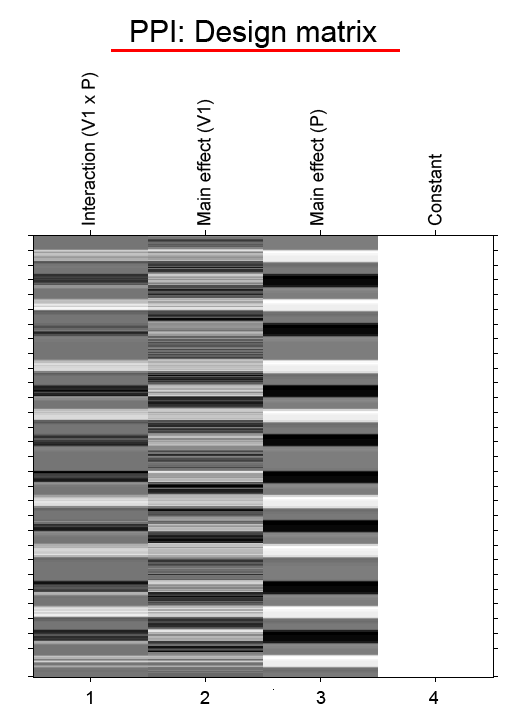
\includegraphics[width=85mm]{ppi/figures/Fig1.png}
	\caption{\em Example design matrix for a PPI (or \((\Phi\)PI)). The main effects are BOLD activity from area V1, in column 2, and a psychological vector, e.g., attention vs. no attention (P), in column 3. Inference would typically focus on the interaction term, in column 1, using a contrast vector of \textsc{[1 0 0 0]}. In \(\Phi\)PIs the third column would be BOLD activity from a second source region rather than the psychological factor.}
	\label{fig:ppi1}
\end{figure}

Both PPIs and $\Phi$PIs can be conceived of as models of ``contribution''. PPIs occupy middle-ground between between models of  functional vs. effective connectivity \cite{ppi}. Functional connectivity (FC) is defined as the temporal correlation between spatially separated neurophysiological events \cite{ppi}. FC analyses are typically model-free and do not specify a direction of influence, i.e., the influence of A on B is indistinguishable from the influence of B on A. In contrast, PPI's are based on regression models, and therefore a direction of influence is chosen based on the model. Effective connectivity (EC) is defined as the influence one neural system has on another \cite{func1}. PPIs are closely related to EC models, but because PPIs are generally very simple (i.e., 1 source region and 1 experimental factor, or 2 source regions in the case of $\Phi$PIs) they are very limited models of EC.

The interaction between the source region and experimental context (or two source regions) can be interpreted in 2 different ways: 1) as demonstrating how the contribution of one region to another is altered by the experimental context or task, or 2) as an example of how an area's response to an experimental context is modulated by input from another region, Figure~\ref{fig:ppi2}.\\

\begin{figure}[!h]
	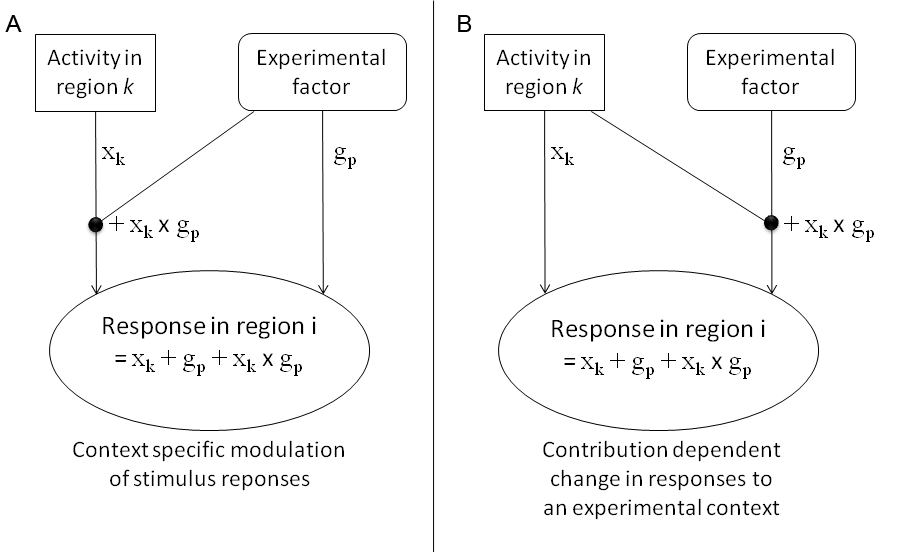
\includegraphics[width=120mm]{ppi/figures/Fig2.png}
	\caption{Two alternative interpretations of PPI effects. A) The contribution of one area (k) to another (i) is altered by the experimental (psychological) context. B) The response of an area (i) to an experimental (psychological) context due to the contribution of region (k). (Adapted from \cite{ppi})}
	\label{fig:ppi2}
\end{figure}

\section{Psycho-Physiologic Interaction Analysis: Summary of Steps}
Mechanistically, a PPI analysis involves the following steps.
\begin{enumerate}
\item Performing a standard GLM analysis.
\item Extracting BOLD signal from a source region identified in the GLM analysis.
\item Forming the interaction term (source signal x experimental treatment)
\item Performing a second GLM analysis that includes the interaction term, the source region's extracted signal and the experimental vector in the design. The inclusion of the source region's signal and the experimental vector is analogous to including the main effects in an ANOVA in order to make an inference on the interaction.
\end{enumerate} 

Forming the proper interaction term turns out to be a challenge because of the unique characteristics of fMRI (BOLD) data in which the underlying neural signal is convolved with a hemodynamic response function. However, interactions in the brain take place at the neural and not the hemodynamic level. Therefore, appropriate models of the interactions require the neural signal, which is not measured directly, but instead must be derived by deconvolving the HRF. The PPI software (\texttt{spm\_peb\_ppi.m}) was developed in order to provide robust deconvolution of the HRF and the proper derivation of the interaction term \cite{gitelman_03}.

\section{Practical example}

The dataset in this exercise is from one subject who was studied in the \cite{buchel1998} report and refers to the ``attention to motion'' dataset available from the SPM website\footnote{\url{http://www.fil.ion.ucl.ac.uk/spm/data/attention/}}. It has already been described in the previous chapter for DCM.

The goal is to use PPI to examine the change in effective connectivity between V2 and V5 while the subject observes visual motion (radially moving dots) under the experimental treatments of attending vs. not attending to the speed of the dots. The psychophysiologic interaction can be conceived of as looking for a significant difference in the regression slopes of V1 vs. V5 activity under the influence of the different attentional states \cite{ppi}.

\subsection{GLM analysis - Design setup and estimation}

This dataset has already been preprocessed (coregistered, normalised and smoothed) using an earlier version of SPM.

\begin{enumerate}
\item The analysis directory should include
\begin{enumerate}
\item A directory named \texttt{functional}, which includes the preprocessed fMRI volumes.
\item A directory named \texttt{structural}, which includes a T1 structural volume
\item Files: \texttt{factors.mat}, \texttt{block\_regressors.mat}, \texttt{multi\_condition.mat} and \linebreak[4] \mbox{\texttt{multi\_\-block\_\-regressors.mat}}.
\item You will also need to make 2 empty directories called \texttt{GLM} and
\texttt{PPI} for performing the analyses.
\end{enumerate}

\item In \matlab\ type
\begin{verbatim}
>> cd GLM
>> spm fmri
\end{verbatim}

\item Start the Batch system by clicking the \textsc{Batch} button. 
\item From the \textsc{SPM} menu in the Batch window, click \textsc{Stats} and then select the modules \textsc{fMRI Model Specification}, \textsc{Model Estimation} and \textsc{Contrast Manager}, Figure~\ref{fig:ppi3}.

\begin{figure}[ht]
\centering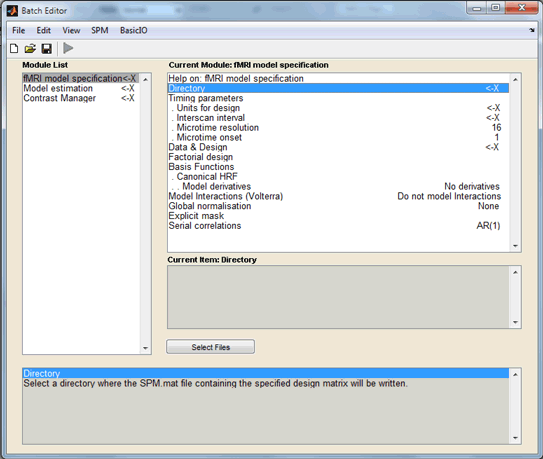
\includegraphics[width=120mm]{ppi/figures/Fig3.png}
\caption{Batch Editor showing the \textsc{fMRI Model Specification}, \textsc{Model Estimation} and \textsc{Contrast Manager} modules.}
\label{fig:ppi3}
\end{figure}

\textbf{Fill in the \textsc{fMRI Model Specification}}

\item Click \textsc{Directory} and choose the \texttt{GLM} directory that you made above.
\item \textsc{Units for design} [\textsc{scans}]
\item \textsc{Interscan interval} [3.22]
\item \textsc{Microtime resolution} [16]
\item \textsc{Microtime onset} [1]
\item Click \textsc{Data \& Design}. Then in the \textsc{Current Item} box click \textsc{New: Subject/Session}, Figure~\ref{fig:ppi4}.

\begin{figure}[!ht]
\centering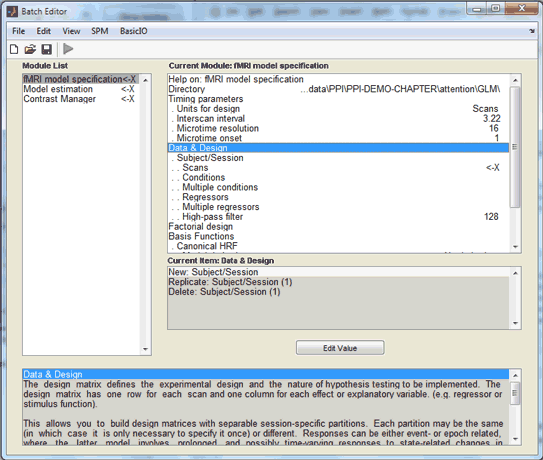
\includegraphics[width=120mm]{ppi/figures/Fig4.png}
\caption{\em Fill in the Data \& Design}
\label{fig:ppi4}
\end{figure}

\item Click \textsc{Scans} and choose all the functional scans \texttt{snffM00587\_00xx.img}. There should be 360 \texttt{*.img} files.
\item The experimental conditions can be defined either individually or using a multiple condition \texttt{mat}-file. This exercise shows both methods for educational purposes. When doing an actual analysis you can just follow one of the two approaches below.\\\\

\textbf{Define conditions individually}
\item Load the mat file containing the individual conditions:
\begin{verbatim}
>> load factors.mat
\end{verbatim}
You can look at the loaded variables by typing the variable names.
( \texttt{stat} = stationary, \texttt{natt} = no attention, \texttt{att} = attention)
\begin{verbatim}
>> stat
>> natt
>> att
\end{verbatim}
\item Click \textsc{Conditions} then in the \textsc{Current Item} box click \textsc{New: Condition} 3 times, Figure~\ref{fig:ppi5}.

\begin{figure}[!ht]
\centering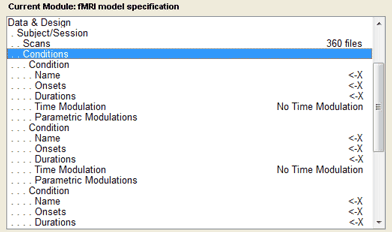
\includegraphics[width=120mm]{ppi/figures/Fig5.png}
\caption{\em \textsc{Current Module} section of the \textsc{Batch Editor} showing 3 Conditions to be filled in.}
\label{fig:ppi5}
\end{figure}

\item Condition 1: Name = \texttt{Stationary}, \textsc{Onsets} = \texttt{stat}, \textsc{Durations} = 10. 
\item Condition 2: Name = \texttt{No-attention}, \textsc{Onsets} = \texttt{natt}, \textsc{Durations} = 10.
\item Condition 3: Name = \texttt{Attention}, \textsc{Onsets} = \texttt{att}, \textsc{Durations} = 10.
\item Next you will enter 3 regressors to model block effects. This will account for the fact that the experiment took place over 4 runs that have been concatenated into a single session to make the PPI analysis easier. {\em Note: Only 3 of the 4 sessions need to be modeled by block regressors because the fourth one is modeled by the mean column of the design matrix.}

First load the regressors:
\begin{verbatim}
>> load block_regressor.mat
\end{verbatim}
\item Click \textsc{Regressors} then click \textsc{New: Regressor} 3 times in the \textsc{Current Item} box, Figure~\ref{fig:ppi6}.

\begin{figure}[!ht]
\centering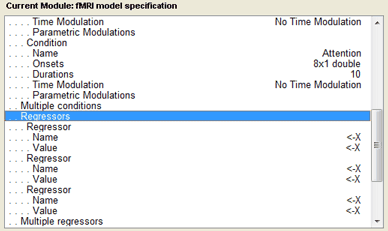
\includegraphics[width=120mm]{ppi/figures/Fig6.png}
\caption{\em \textsc{Current Module} section of the \textsc{Batch Editor} showing 3 Regressors to be filled in.}
\label{fig:ppi6}
\end{figure}

\item Regressor 1: \textsc{Name} = \texttt{Block 1}, \textsc{Value} = \texttt{block1}
\item Regressor 2: \textsc{Name} = \texttt{Block 2}, \textsc{Value} = \texttt{block2}
\item Regressor 3: \textsc{Name} = \texttt{Block 3}, \textsc{Value} = \texttt{block3}\\\\

\textbf{Define conditions using multiple condition and multiple regressor files}
\item If you would like to look at the organization of the variables in the multiple condition file, first load it.
\begin{verbatim}
>> load multi_condition.mat
>> names
>> onsets
>> durations
\end{verbatim}
The variables in a multiple condition file must always be named: 'names', 'onsets', and 'durations'. Notice that these three variables are cell arrays.
\textit{(Note: You only need to do this step if you want to look at the organization of the variables. In contrast to defining conditions individually, as shown above, when using a multiple condition file you do not have to load the file in order to enter it into the design.)}\\
\item To use the multiple conditions file in the design, click \textsc{Multiple Conditions}, then \textsc{Specify Files} in the Options box and choose the \texttt{multi\_condition.mat} file.
\item Next you will enter the 3 regressors to model block effects by using a multiple regressor file. To look at the organization of the multiple regressor variable, first load it. \textit{(Again you do not have to load the multiple regressor file in order to use it. This step is just to allow you to examine the file and the variables it contains.)}
\begin{verbatim}
>> load multi_block_regressor.mat
>> R
\end{verbatim}
Notice that this file contains a single variable, \texttt{R}, which is a 360 x 3 matrix. The number of rows is equal to the number of scans, and each regressor is in a separate column.
\item To use the multiple regressor file, click \textsc{Multiple Regressors} then select the  \texttt{multi\_\-block\_\-regressor.mat} file.\\\\

\textbf{Complete the design setup}
\item \textsc{High-pass filter} [192] (Note: most designs will use a high-pass filter value of 128. However, this dataset requires a longer high-pass filter in order not to lose the low frequency components of the design.)
\item \textsc{Factorial design} is not used
\item The \textsc{Basis function} is the \textsc{canonical HRF} as shown and \textsc{Model derivatives} [\textsc{No derivatives}]
\item \textsc{Model Interactions (Volterra)}: [\textsc{Do not model interactions}]
\item \textsc{Global normalisation} [\textsc{None}]
\item \textsc{Explicit mask} [\textsc{None}]
\item \textsc{Serial correlations} [\textsc{AR(1)}]\\\\

\textbf{Model Estimation}
\item Under \textsc{Model estimation} click \textsc{Select \texttt{SPM.mat}} then click the \textsc{Dependency} button and choose \textsc{fMRI model specification: SPM.mat File}. The \textsc{Method} should be left as Classical.\\\\

\textbf{Contrast Manager}
\item Under \textsc{Contrast Manager} click \textsc{Select \texttt{SPM.mat}} then click the \textsc{Dependency} button and choose \textsc{Model estimation: SPM.mat File}

\item Click \textsc{Contrast Sessions} then click \textsc{New: F-contrast} once, and \textsc{New: T-contrast} twice from the \textsc{Current Item} box.
\item Click \textsc{Contrast vectors} and then \textsc{New: F contrast vector}. 
\item The F contrast vector can be entered as [eye(3), zeros(3,4)], which will produce:
\begin{verbatim}
1 0 0 0 0 0 0
0 1 0 0 0 0 0
0 0 1 0 0 0 0
\end{verbatim}

\item For the first T-contrast, \textsc{Name} is \texttt{Attention}, and the \textsc{T contrast vector} is \texttt{~0~-1~1~0~0~0~0} (Note the order of the conditions in the design matrix is: Stationary, NoAttMot and AttMot).
\item For the second T-contrast \textsc{Name} is \texttt{Motion}, and the \textsc{T contrast vector} is: \texttt{-2~1~1~0~0~0~0}.

\item Click the \textsc{Save} icon on the toolbar and save the batch file.\\

\textbf{Design estimation}\\
\item If everything has been entered correctly the \textsc{Run} button should now be green. Click \textsc{Run} to estimate the design.
\item The design matrix should look as shown in Figure~\ref{fig:ppi7}, below.

\begin{figure}[!ht]
\centering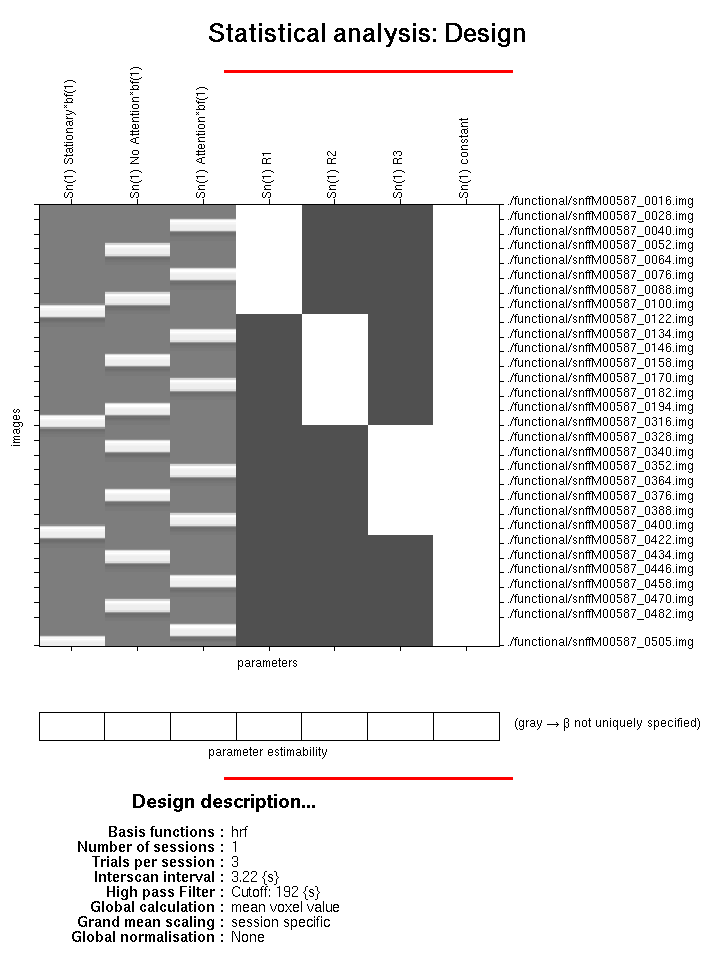
\includegraphics[width=85mm]{ppi/figures/Fig7.png}
\caption{\em Design matrix}
\label{fig:ppi7}
\end{figure}
\end{enumerate}

\subsection{GLM analysis - Results}

\begin{enumerate}
\item Click \textsc{Results} and select the \texttt{SPM.mat} file.
\item Choose the \texttt{Attention} contrast
\item Mask with other contrasts [No]
\item Title for comparison [Attention]
\item p value adjustment to control [None]
\item threshold {T or p value} [0.0001]
\item \& extent threshold {voxels} [10]
\item You should see an SPM that looks like the one shown below, Figure~\ref{fig:ppi8}. Note the Superior Parietal and Dorso-Lateral Prefrontal activations, among others. By selecting \textsc{overlays} $\rightarrow$ \textsc{sections}, and selecting the normalised structural image, you should be able to identify the anatomy more accurately.

\begin{figure}[!ht]
\centering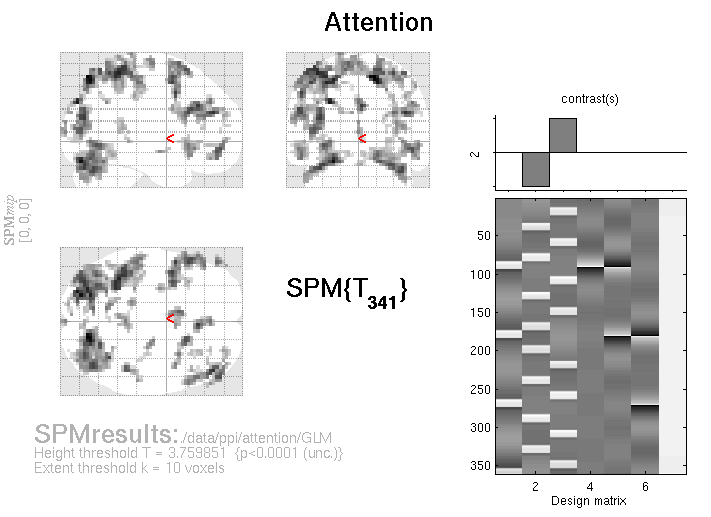
\includegraphics[width=85mm]{ppi/figures/Fig8.png}
\caption{\em Statistical parametric map for the \texttt{Attention} contrast}
\label{fig:ppi8}
\end{figure}

\item To look at the \texttt{Motion} contrast where \texttt{Attention} is greater than \texttt{No Attention}, click \textsc{Results}, choose the \texttt{SPM.mat} file and choose the \texttt{Motion} contrast.
\item apply masking [Yes]
\item Select contrast for masking: Choose the \texttt{Attention} contrast
\item Uncorrected mask p-value [0.01]
\item Nature of Mask: [inclusive]
\item title for comparison: leave as the defaults, which is [Motion  (masked [incl.] by Attention at p=0.01)]
\item p value adjustment to control [FWE]
\item threshold {T or p value} [0.05]
\item \& extent threshold {voxels} [3]
\item The masked \texttt{motion} contrast on the glass brain is shown below in Figure~\ref{fig:ppi9}.

\begin{figure}[!ht]
\centering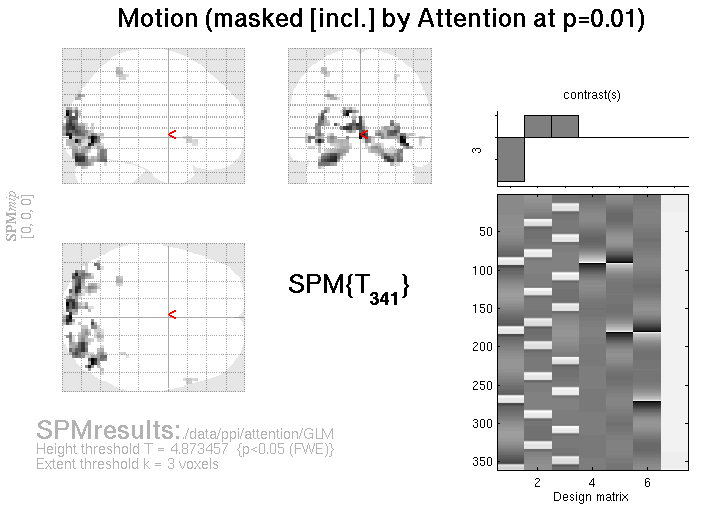
\includegraphics[width=85mm]{ppi/figures/Fig9.png}
\caption{\em Statistical parametric map for the \texttt{Motion} contrast inclusively masked by the Attention contrast}
\label{fig:ppi9}
\end{figure}
\end{enumerate}

\section{GLM analysis - Extracting VOIs}

\begin{enumerate}
\item First select the \texttt{Motion} contrast, but do not include masking. Use a p-value adjustment of FWE with height threshold of 0.05 and a cluster threshold of 3.
\item Go to point [15 -78 -9]
\item Press \texttt{eigenvariate}
\item Name of region [V2]
\item Adjust data for [effects of interest]
\item VOI definition [sphere]
\item VOI radius(mm) [6]
\end{enumerate}
This saves the extracted VOI data in the file \texttt{VOI\_V2\_1.mat} in the working directory, and displays Figure~\ref{fig:ppi10}, below. The left side shows the location on a standard brain. The right side shows the first eigenvariate of the extracted BOLD signal. 

\begin{figure}[!ht]
\centering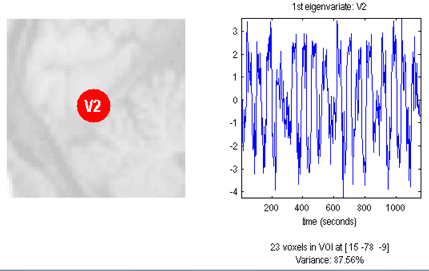
\includegraphics[width=85mm]{ppi/figures/Fig10.png}
\caption{\em First eigenvariate of the extracted BOLD signal in V2}
\label{fig:ppi10}
\end{figure}

\section{PPI analysis - Create PPI variable\label{create_ppi}}
\begin{enumerate}
\item PPIs can be calculated either by pressing the \textsc{PPIs} button in the \textsc{SPM Menu} window, or by selecting the \textsc{Physio/Psycho-Physiologic} menu item from the SPM $\rightarrow$ Stats menu of the \textsc{Batch Editor}. This example uses the \textsc{Batch Editor}, Figure~\ref{fig:ppi11}.

\begin{figure}[!ht]
\centering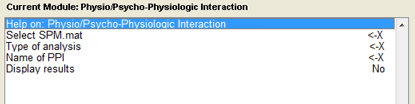
\includegraphics[width=100mm]{ppi/figures/Fig11.png}
\caption{\em Physio/Psycho-Physiologic module in the Batch Editor}
\label{fig:ppi11}
\end{figure}

\item Choose the \textsc{SPM.mat} file in the \texttt{GLM} directory.
\item Type of analysis: Choose \textsc{Psycho-Physiologic interaction}, Figure~\ref{fig:ppi12}.

\begin{figure}[!ht]
\centering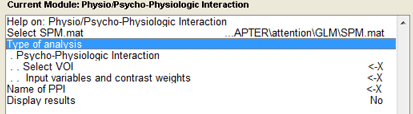
\includegraphics[width=100mm]{ppi/figures/Fig12.png}
\caption{\em Specifying a Psycho-Physiologic interaction.}
\label{fig:ppi12}
\end{figure}

\item Select VOI: Choose \texttt{VOI\_V2\_1.mat}
\item Input variables and contrast weights: Must be specified as an n x 3 matrix, where n is the number of conditions included in the PPI. The first column of the matrix indexes SPM.Sess.U(i). The second column indexes SPM.Sess.U(i).name{ii}. It will generally be a 1 unless there are parametric effects. The third column is the contrast weight. In order to include Attention - No-attention in the PPI, recall that the conditions were entered as: Stationary, No-attention, Attention, therefore the matrix should be.
\begin{verbatim}
[2 1 -1; 3 1 1]
\end{verbatim}
\item Name of PPI [ V2x(Att-NoAtt) ]
\item Display results: Yes
\end{enumerate}

After a few seconds the PPI will be calculated and a graphical window will appear, Figure~\ref{fig:ppi13}. In the upper left, the details of the PPI setup calculation are given including the name of the PPI, the chosen VOI file, and the included conditions and their contrast weights. The main central graph shows the original BOLD signal (actually the eigenvariate) in blue and the neuronal or deconvolved signal in green. These will look quite similar for block design data. The graph in the lower left shows the task condition plot, dotted green line, and the convolved task conditions (psych variable). In the lower right the PPI interaction term is plotted.

\begin{figure}[!ht]
\centering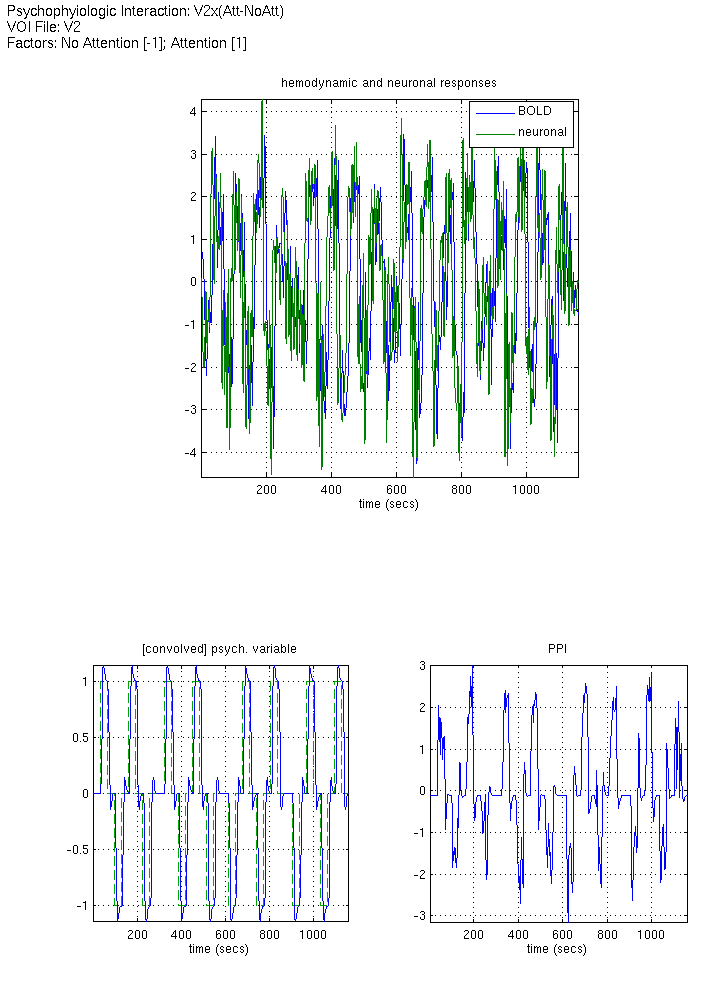
\includegraphics[width=100mm]{ppi/figures/Fig13.png}
\caption{\em PPI output graphics}
\label{fig:ppi13}
\end{figure}

The PPI calculation will create a file \texttt{PPI\_V2x(Att-NoAtt).mat} in the current working directory. It contains the variable \texttt{PPI.ppi} (the interaction term), \texttt{PPI.Y} (the original VOI eigenvariate) and \texttt{PPI.P} (the \texttt{Attention - No Attention} task vector). You will use these vectors in setting up your psychophysiologic interaction GLM analysis. See \texttt{spm\_peb\_ppi} for a full description of the \texttt{PPI} data structure. 

\subsection{PPI GLM analysis - Design setup and estimation}

\begin{enumerate}
\item Copy the file \texttt{PPI\_V2x(Att-NoAtt)} \textsc{Mat}-file to the \texttt{PPI} directory that you created at the start of this exercise.
\item Change directory to the new one, i.e. \texttt{cd PPI}
\item At the \matlab\ prompt type
\begin{verbatim}
>> load PPI_V2x(Att-NoAtt)
\end{verbatim}

\item In the \textsc{Batch Editor} setup another GLM analysis by choosing the modules \textsc{fMRI Model Specification}, \textsc{Model Estimation} and \textsc{Contrast Manager} as you did above, and fill it in as follows.
\item Directory: Choose the \texttt{PPI} directory
\item Units for design [scans]
\item Interscan interval [3.22]
\item Add a \textsc{New: Subject/Session} under \textsc{Data \& Design}
\item Click \textsc{Scans} and choose all the functional scans \texttt{snffM00587\_00xx.img}. There should be 360 \texttt{*.img} files.
\item Click \textsc{New: Regressor} and add 6 regressors.
\item Regressor 1: \textsc{Name} = \texttt{PPI-interaction}, \textsc{Value} = \texttt{PPI.ppi}
\item Regressor 2: \textsc{Name} = \texttt{V2-BOLD}, \textsc{Value} = \texttt{PPI.Y}
\item Regressor 3: \textsc{Name} = \texttt{Psych\_Att-NoAtt}, \textsc{Value} = \texttt{PPI.P}
\item Regressor 4: \textsc{Name} = \texttt{Block 1}, \textsc{Value} = \texttt{block1}
\item Regressor 5: \textsc{Name} = \texttt{Block 2}, \textsc{Value} = \texttt{block2}
\item Regressor 6: \textsc{Name} = \texttt{Block 3}, \textsc{Value} = \texttt{block3}
\item High Pass Filter [192]\\\\

\textbf{Model Estimation}
\item Under \textsc{Model estimation} click \textsc{Select \texttt{SPM.mat}} then click the \textsc{Dependency} button and choose \textsc{fMRI model specification: SPM.mat File}. The \textsc{Method} should be left as Classical.\\\\

\textbf{Contrast Manager}
\item Under \textsc{Contrast Manager} click \textsc{Select \texttt{SPM.mat}} then click the \textsc{Dependency} button and choose \textsc{Model estimation: SPM.mat File}
\item Click \textsc{Contrast Sessions} then click \textsc{New: T-contrast}
\item T-contrast, \textsc{Name}: \texttt{PPI-Interaction}, vector: \texttt{1~0~0~0~0~0~0}
\item Save the batch file.
\item Run
\end{enumerate}
The design matrix is shown below, Figure~\ref{fig:ppi14}.

\begin{figure}[ht]
\centering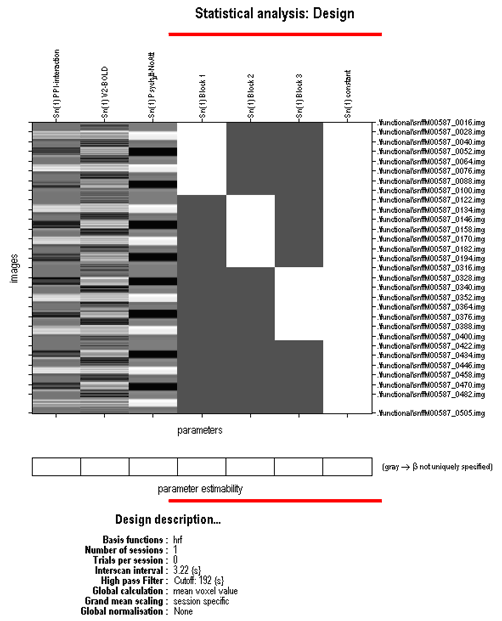
\includegraphics[width=85mm]{ppi/figures/Fig14.png}
\caption{\em Design matrix for the PPI analysis}
\label{fig:ppi14}
\end{figure}

\subsection{PPI analysis - Results}

\begin{enumerate}
\item Press the \textsc{Results} button and select the \texttt{SPM.mat} file in the PPI directory.
\item Choose the \texttt{PPI-Interaction} contrast
\item apply masking [No]
\item title for comparison [PPI-Interaction]
\item p value adjustment to control [None]
\item threshold {T or p value} [0.01]
\item \& extent threshold {voxels} [10]
\item You should see an SPM that looks the same as the one shown below in the top part of Figure~\ref{fig:ppi15}. The resulting SPM shows areas showing differential connectivity to V2 due to the effect of attention vs. no attention conditions. The effect in this subject is weak.
\end{enumerate}

\begin{figure}[!ht]
\centering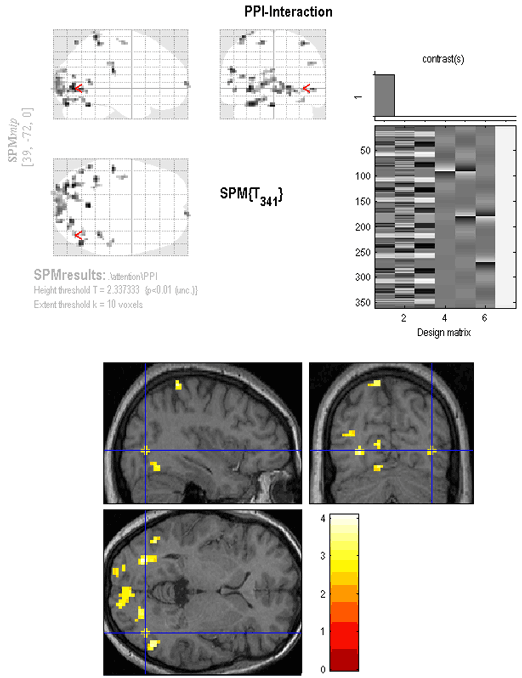
\includegraphics[width=100mm]{ppi/figures/Fig15.png}
\caption{\em PPI results}
\label{fig:ppi15}
\end{figure}

\subsection{PPI analysis - Plotting}
\begin{enumerate}
\item One region showing the psychophysiologic interaction is the V5region, which is located at [39~-72~0] in this subject. Move the cursor to this point to view the area of activation, as shown below, in the bottom half of Figure~\ref{fig:ppi15}.

\item In order to plot the PPI graph showing the effect of attention, you need to extract a VOI from the V5 region. To do this, you will return to the original GLM analysis.
\item Click Results, then select the GLM analysis \texttt{SPM.mat} file and the \texttt{Motion} contrast.
\item apply masking [No]
\item title for comparison [Motion]
\item p value adjustment to control [None]
\item threshold {T or p value} [0.001]
\item \& extent threshold {voxels} [3]
\item Go to point [39~-72~0]
\item Press eigenvariate
\item Name of region [V5]
\item Adjust data for [effects of interest]
\item VOI definition [sphere]
\item VOI radius(mm) [6]
\item Now you will create 4 PPIs (Follow the steps under section~\ref{create_ppi}, Create PPI Variable, above). By using the PPI software machinery to create the interaction vectors, rather than just multiplying the extracted V2 and V5 eigenvariates by the behavioral vectors, the PPI vectors will be formed properly.

\item \texttt{V2xNoAttention} (Use the V2 VOI and include \texttt{No-Attention} with a contrast weight of 1, do not include \texttt{Stationary}, \texttt{Attention})
\item \texttt{V2xAttention} (Use the V2 VOI and include \texttt{Attention} with a contrast weight of 1, do not include \texttt{Stationary}, \texttt{No-Attention})
\item \texttt{V5xNoAttention} (Use the V5 VOI and include \texttt{No-Attention} with a contrast weight of 1, do not include \texttt{Stationary}, \texttt{Attention})
\item \texttt{V5xAttention} (Use the V5 VOI and include \texttt{Attention} with a contrast weight of 1, do not include \texttt{Stationary}, \texttt{No-Attention})

\item Load the PPIs you just created with the following commands at the \matlab\ prompt:
\begin{verbatim}
>> v2noatt = load('PPI_V2xNoAttention');
>> v2att   = load('PPI_V2xAttention.mat');
>> v5noatt = load('PPI_V5xNoAttention.mat');
>> v5att   = load('PPI_V5xAttention.mat');
\end{verbatim}
\item Plot the PPI datapoints with the following commands at the \matlab\ prompt:
\begin{verbatim}
>> figure
>> plot(v2noatt.PPI.ppi,v5noatt.PPI.ppi,'k.');
>> hold on
>> plot(v2att.PPI.ppi,v5att.PPI.ppi,'r.');
\end{verbatim}
\item To plot the best fit lines type the following first for \texttt{NoAttention}
\begin{verbatim}
>> x  = v2noatt.PPI.ppi(:);
>> x  = [x, ones(size(x))];
>> y  = v5noatt.PPI.ppi(:);
>> B  = x\y;
>> y1 = B(1)*x(:,1)+B(2);
>> plot(x(:,1),y1,'k-');
\end{verbatim}
\item Then for \texttt{Attention}
\begin{verbatim}
>> x = v2att.PPI.ppi(:);
>> x = [x, ones(size(x))];
>> y = v5att.PPI.ppi(:);
>> B = x\y;
>> y1 = B(1)*x(:,1)+B(2);
>> plot(x(:,1),y1,'r-');
>> legend('No Attention','Attention')
>> xlabel('V2 activity')
>> ylabel('V5 response')
>> title('Psychophysiologic Interaction')
\end{verbatim}
\end{enumerate}

\begin{figure}[!ht]
\centering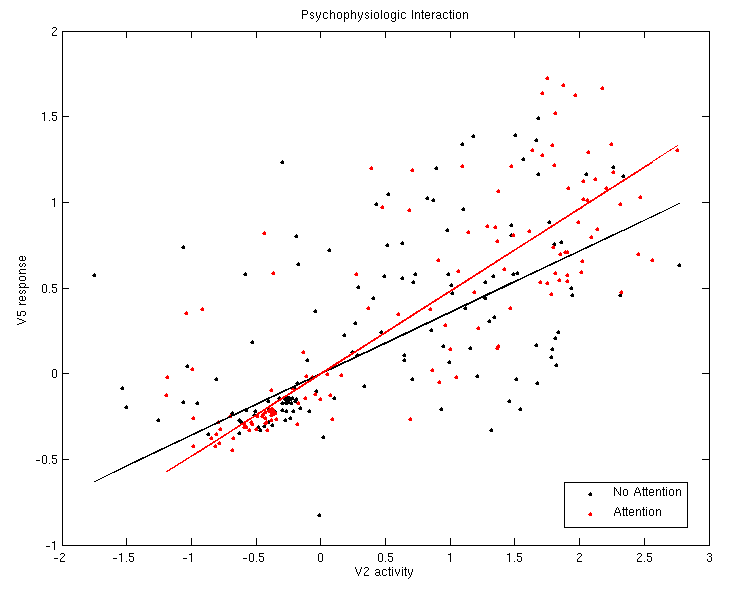
\includegraphics[width=85mm]{ppi/figures/Fig16.png}
\caption{\em Graph demonstrating PPI interaction.}
\label{fig:ppi16}
\end{figure}
